% Author: Mick van Gelderen
% Created from http://www.texample.net/tikz/examples/class-diagram/ and other examples and resources. 

%\documentclass{standalone}
%\usepackage{tikz}
\usetikzlibrary{calc,positioning,shapes,arrows,decorations.pathreplacing}
\usetikzlibrary{shapes.multipart}


%\begin{document}




\newcommand{\activity}[3]{\node (v#1) [activity, text width=#2cm, #3] {$v_#1$};}

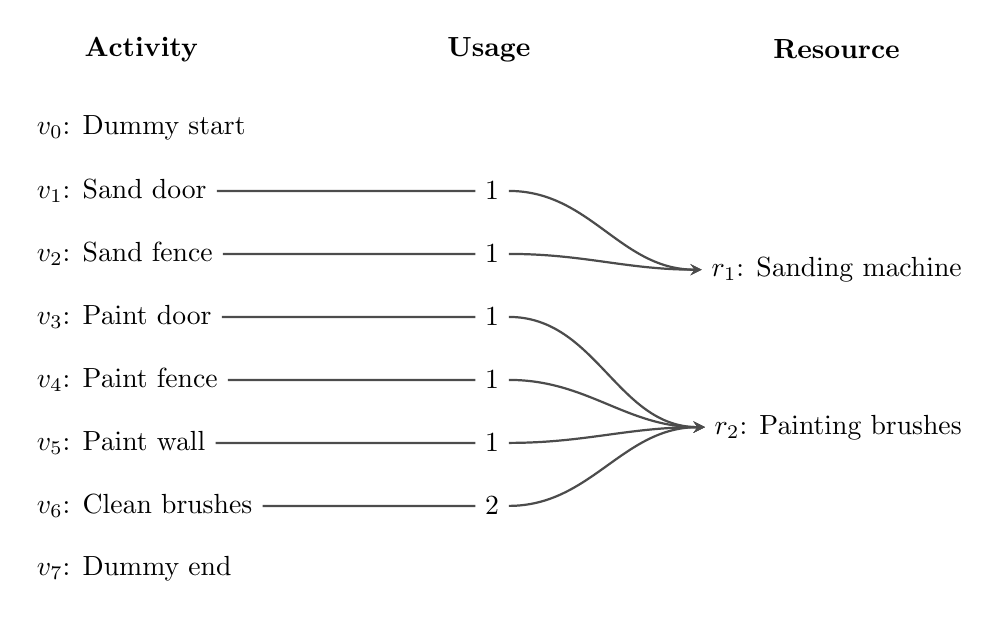
\begin{tikzpicture}[node distance=.8cm]
	\tikzstyle{activity}=[text centered, text=black, thick, minimum height=1.8em, minimum width=1.8em]
	\tikzstyle{resource}=[text centered]
	\tikzstyle{header}=[font=\bfseries]
	\tikzstyle{usage}=[->,>=stealth, draw=black!70, thick]

	\node (v0) [activity] {$v_0$: Dummy start};
	\node (v1) [activity, below=of v0.west, anchor=west] {$v_1$: Sand door};
	\node (v2) [activity, below=of v1.west, anchor=west] {$v_2$: Sand fence};
	\node (v3) [activity, below=of v2.west, anchor=west] {$v_3$: Paint door};
	\node (v4) [activity, below=of v3.west, anchor=west] {$v_4$: Paint fence};
	\node (v5) [activity, below=of v4.west, anchor=west] {$v_5$: Paint wall};
	\node (v6) [activity, below=of v5.west, anchor=west] {$v_6$: Clean brushes};
	\node (v7) [activity, below=of v6.west, anchor=west] {$v_7$: Dummy end};
	
	\node (u1) [right=5.7cm of v1.west] {1};
	\node (u2) [right=5.7cm of v2.west] {1};
	\node (u3) [right=5.7cm of v3.west] {1};
	\node (u4) [right=5.7cm of v4.west] {1};
	\node (u5) [right=5.7cm of v5.west] {1};
	\node (u6) [right=5.7cm of v6.west] {2};

	\coordinate (mid) at ($(v0.west)!.5!(v7.west) + (12,0)$);
	\node (r1) [resource, above=1cm of mid, anchor=east] {$r_1$: Sanding machine};
	\node (r2) [resource, above=-1cm of mid, anchor=east] {$r_2$: Painting brushes};

	\draw let \p1 = (v0), \p2 = (r1) in 
		node (ac) [header] at ($(\x1,\y1) + (0,1)$) {Activity}
		node (res) [header] at ($(\x2,\y1) + (0,1)$) {Resource};
	\node (us) [header] at ($(ac)!.5!(res)$) {Usage};
	
  \draw[usage] (v1.east) -- (u1) to[out=0,in=180] (r1.west);
  \draw[usage] (v2.east) -- (u2) to[out=0,in=180] (r1.west);
  \draw[usage] (v3.east) -- (u3) to[out=0,in=180] (r2.west);
  \draw[usage] (v4.east) -- (u4) to[out=0,in=180] (r2.west);
  \draw[usage] (v5.east) -- (u5) to[out=0,in=180] (r2.west);
  \draw[usage] (v6.east) -- (u6) to[out=0,in=180] (r2.west);

  
	
\end{tikzpicture}

%\end{document}